\subsection{Sphinxes: the Sphinx header format Extended for Sets of nodes}%
\label{Sphinxes}

\Textcite{Sphinx} designed \iac{UC} secure message format for mixes, called 
Sphinx.
Since it is \ac{UC} secure, it provably implements an ideal onion routing 
functionality.
\Ie, it provides bitwise unlinkability on the forward route, hides the path 
length, makes replies indistinguishable from forward messages and resists 
tagging attacks.
It is also compact with only 224 bytes of header for a five-hop path with 
128-bit security.
Sphinx only provides one node per onion layer, in this section we extend Sphinx 
to Sphinxes, which allows for multiple nodes per onion layer.
(See \cref{fig:OR-POR}.)

\begin{figure}
  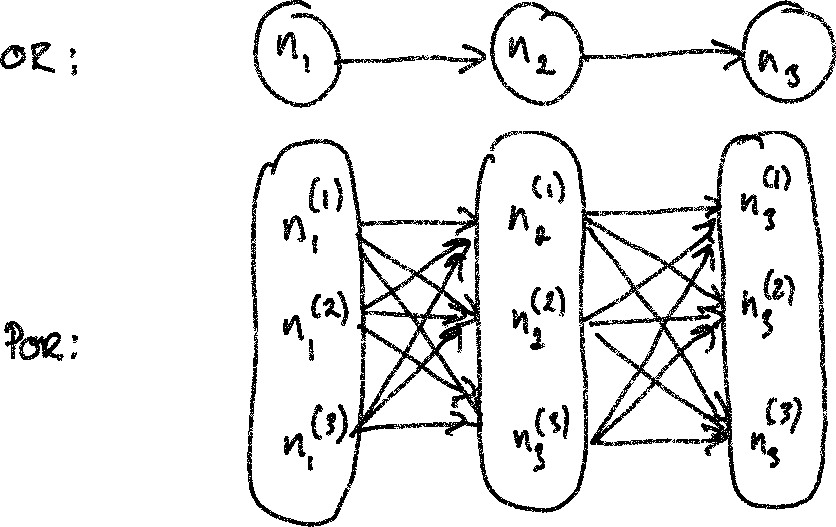
\includegraphics[width=\linewidth]{figures/OR-POR.png}
  \caption{\label{fig:OR-POR}%
    Illustration of the conceptual difference to traditional onion routing and 
    mixing.
  }
\end{figure}

\subsubsection{Overview of the Sphinx header format}

We will now give an overview of the Sphinx header format.
The idea is not to give a detailed description of Sphinx, but to to give the 
reader enough understanding of Sphinx to understand the changes we make to 
achieve Sphinxes.
For a more detailed understanding of Sphinx, we refer the reader to the 
excellent description in the original Sphinx paper~\cite{Sphinx}.

\NewVariable{\sk}{x}
\NewVariable{\pk}{X}

Each node \(n\) in the system has a long-term public-key pair: private key 
\(\sk_n\in \ZZ_q^*\) and public key \(\pk_n = g^{\sk_n}\in G\), where \(g\) 
generates a group \(G\) of prime order \(q\).

The Sphinx header (for the first node) is a triple \((\alpha_1, \beta_1, 
  \gamma_1)\), where \(\alpha_1\) is \iac{DHKE} exponent (\(g^x\), where \(x\) 
is a short-term secret chosen randomly for each header), \(\beta_1\) is the 
encrypted routing data and \(\gamma_1\) is \iac{MAC} for \(\beta_1\).
The payload data, \(\delta\), is treated separately from the header.

The first node in the path, with keys \((\pk_1, \sk_1)\), will compute the 
shared secret \(s_1 = \alpha_1^{\sk_1}\), \ie complete the \ac{DHKE} round.
Since \(\pk_1\) is an authenticated key, the sender can be sure that only this 
particular node can process the first layer of the onion.

The derived shared secret \(s_1\) is then used to derive various keys.
One of them is the key for the \ac{MAC} (\(gamma_1\)) to verify the integrity 
of the header (\(\beta_1\)).
If \(\beta_1\) is correct, another key is derived from \(s_1\) to decrypt 
\(\beta_1\) to get \(d_2\concat \gamma_2\concat \beta_2\), where \(d_2\) is the 
address of the second node in the path.

We note that \(\beta_i\) is encrypted using a stream cipher.
Thus we can append zeroes before decryption to keep the ciphertext length 
constant.
Since we append \emph{before} decryption, those appended zeroes will look 
completely random to the next node, thus the position on the path is hidden.

Finally, \(\alpha_1\) is blinded into \(\alpha_2\) with a key derived from 
\(s_1\).
Then the triple \((\alpha_2, \beta_2, \gamma_2)\) are sent to the node with 
address \(d_2\).

When node \(n\) discovers \(d_{n+1} = *\) it knows that the message is intended 
for itself and thus stops the forwarding.

\subsubsection{The Sphinxes extension for sets of nodes}

\NewAlgorithm{\Enc}{Enc}

We will now extend Sphinx to do \ac{POR}: instead of providing only \(d_{i+1}\) 
in \(\beta_i\), we will have a set \(\{d_{i+1}^{(0)}, \dotsc, d_{i+1}^{(m)}\}\) 
of \(m\) alternative next nodes.
This means that all \(m\) nodes must be able to compute the same shared secret 
\(s_{i+1}\).
We do this by adding one layer of indirection.

In Sphinx we denoted the public key for layer \(i\) as \(\pk_i\).
Since we have \(m\) alternative nodes with different keys, let us denote them 
by \(\pk_i^{(1)}, \dotsc, \pk_i^{(m)}\).

We extend the header to a quadruple \((\alpha_i, C_i, \beta_i, \gamma_i)\), 
where \(\alpha_i, \beta_i, \gamma_i\) are the same as before.
We let the shared secret \(s_i\) be chosen uniformly randomly instead of being 
computed as \(\alpha_i^{\sk_i}\).
We now compute one shared secret per alternative node, \ie \(s_i^{(j)} = 
  \alpha_i^{\sk_i^{(j)}}\) for \(1\leq j\leq m\).
Then \(C_i = c_i^{(1)}\concat \dotsb\concat c_i^{(m)}\) is the concatenation of 
ciphertexts \(c_i^{(j)} = \Enc[_{s_i^{(j)}}][s_i]\), where \(\Enc\) is 
\iac{SKE} algorithm and each ciphertext contains the shared secret \(s_i\) 
encrypted under the individual keys \(s_i^{(j)}\). 

When a node receives this new header, it will compute \(s_i^{(j)}\gets 
  \alpha_i^{\sk_i^{(j)}}\).
Then, it will try to decrypt each ciphertext component \(c_i^{(k)}\) of \(C_i\) 
to get \(\hat s_i\).
If \iac{MAC} key that successfully verifies \(\beta_i\) using \(\gamma_i\) can 
be derived from \(\hat s_i\), then the node knows that \(\hat s_i = s_i\).


\subsubsection{Sphinxes algorithms and \acf*{POR}}

\NewScheme{\Sphinxes}{POR}
\NewAlgorithm{\CreateHeader}{\Sphinxes[CreateHeader]}
\NewAlgorithm{\WrapHeader}{\Sphinxes[WrapHeader]}
\NewAlgorithm{\AttachPayload}{\Sphinxes[AttachPayload]}
\NewAlgorithm{\Process}{\Sphinxes[Process]}

Sphinxes provides the following algorithms:
\begin{itemize}
  \item \(\CreateHeader\) creates a header, this is a modification of that of 
    Sphinx~\cite[\S 3.2, \S 3.4]{Sphinx}.
  \item \(\WrapHeader\) is used to wrap a given single-use reply block given 
    the proper keys.
  \item \(\AttachPayload\) attaches a payload to the header, \ie makes it 
    sendable.
    This is what Sphinx~\cite[\S 3.3]{Sphinx} calls a forward message.
  \item \(\Process\) is the algorithm for processing incoming messages, the 
    processing is identical to Sphinx~\cite[\S 3.6, \S 3.7]{Sphinx} but uses a 
    different interface.
\end{itemize}

\NewVariable{\G}{\mathcal{G}}
\NewVariable{\mac}{\mu}
\NewVariable{\prg}{\rho}
\NewVariable{\prp}{\pi}
\NewVariable{\hash}{h}
%\NewVariable{\tag}{\tau}
\NewVariable{\blind}{b}
\NewVariable{\N}{\mathcal{N}}
\NewVariable{\D}{\mathcal{D}}

We will synchronize our detailed descriptions with that of 
Sphinx~\cite{Sphinx}, hence we will use the following notation:
\begin{itemize}
  \item \(\kappa\) is the security parameter.
    The adversary must thus do about \(2^\kappa\) work to break the security.

  \item \(r\) is the maximum number of nodes (\ie equivalent to the number of 
    layers) that a message will traverse before reaching its destination.

  \item \(\G\) is a prime-order cyclic group satisfying the \ac{DH} assumption.

  \item \(\mac\colon \bin^\kappa\times \bin^*\to \bin^\kappa\) is \iac{MAC}.
    It can be instantiated as \eg SHA256-HMAC-128.

  \item \(\prg\colon \bin^\kappa\to \bin^{(2r+3)\kappa}\) is \iac{PRG}.
    It can be instantiated as any block cipher in counter mode.

  \item \(\prp\colon \bin^\kappa\times \bin^{l_\prp} \to \bin^{l_\prp}\) is 
    \iac{PRP}.
    It can be instantiated using the LIONESS block cipher~\cite{LIONESS}.

  \item \(\hash_\mac, \hash_\prg, \hash_\prp\) are all distinct hash functions 
    of the form \(\bin^\kappa\to \bin^\kappa\).
    They are used as key-derivation functions.

  \item \(\hash_\tau\colon \G^*\to \bin^{2\kappa}\) is used to identify 
    previously seen elements of \(\G^*\).

  \item \(\hash_\blind\colon \G^*\times \G^*\to \ZZ_q^*\) is used to compute 
    blinding factors.
    All the hash functions can be instantiated with truncated versions of hash 
    functions from the SHA-2 and -3 families.

  \item \(\N\subset \bin^\kappa\) is a set of node identifiers.
    Each node \(n\in \N\) has a private key \(\sk_n\in \ZZ_q^*\) and a public 
    key \(\pk_n = g^{\sk_n}\in \G^*\).
    We assume that the identifier--public-key pairs, \((n, \pk_n)\), are 
    distributed.
    (Sphinx made a difference between nodes and destinations, \ie the set 
    \(\D\) such that \(\D\cap \N = \emptyset\) and \(\D\cup \N\) is prefix 
    free, see~\cite{Sphinx} for details.
    We could do the same adoption, but we do not need that for the purposes of 
    this paper.)
    We let \(*\in \N\) be the special identifier of the null node.

  \item \(0_x\) denotes \(x\) zeroes.
    \(s_{[a..b]}\) denotes all bits from the \(a\)th bit to the \(b\)th of the 
    bit string \(s\).
\end{itemize}

\NewAlgorithm{\ComputeKeys}{ComputeKeys}
\NewAlgorithm{\ComputePadding}{ComputePadding}

The \(\CreateHeader\) algorithm is based on that of Sphinx~\cite[\S 
3.2]{Sphinx}.

\Cref{fig:CreateHeader} summarizes the algorithm.
\(w_L\) is the maximum width of a layer, \ie alternative nodes.
\(w_H\) is the header width:
layer nodes' ciphertexts and addresses ($2w_L\kappa$),
address of next node ($\kappa$),
\ac{MAC} ($\kappa$).

We reveal the maximum number of alternatives per layer.
But we do this in ordinary \ac{OR} too, since there is only one node per layer.

First we generate all the needed keys.

\begin{figure*}
  \framebox{\begin{minipage}{0.96\linewidth}
  \begin{algorithmic}[1]
    \Function{\CreateHeader}{$I, L$}
      \State $w_L\gets \max_{N\in L} |N|$
      \Comment{Layer width}
      \State $w_H\gets (2w_L+2)$
      \Comment{Header width}
      \State $(\alpha_0, s_0, C_0, b_0), \dotsc, (\alpha_\nu, s_\nu, C_\nu, 
      b_\nu)\gets \ComputeKeys[L, w_L]$
      \State $\phi_0, \dotsc, \phi_\nu\gets \ComputePadding[\{s_0, \dotsc, 
      s_\nu\}, w_H]$
      \State $\alpha \gets \alpha_\nu$
      \State $C\gets C_\nu$
      \State $\beta \gets
      \left\{\left\{N_\nu\concat
          I\concat
          0_{(2w_L(r-\nu)+2)\kappa}\right\} \oplus
        \prg(\hash_\prg(s_\nu)_{[0..(2w_L(r-\nu)+3)\kappa-1]}\right\}\concat 
      \phi_\nu$
      \Comment{$\beta_\nu$}
      \State $\gamma \gets \mac(\hash_\mac(s_\nu), \beta)$
      \Comment{$\gamma_\nu$}
      \For{$\nu-1\leq i\leq 1$}
        \State $(\alpha, C, \beta, \gamma) \gets
          \WrapHeader[i, (\alpha, \beta, \gamma), \alpha_i, s_i, C_i, N_{i+1}, 
          w_L]$
      \EndFor
      \State \Return $(\alpha, C, \beta, \gamma)$
    \EndFunction

    \Function{\WrapHeader}{$i, (\alpha_{i+1}, \beta_{i+1}, \gamma_{i+1}), 
      \alpha_i, s_i, C_i, N_{i+1}, w_L$}
      \If{$i < 0$}
        \Return $\bot$
      \EndIf
      \State $\beta_i \gets \{N_{i+1}, \concat \gamma_{i+1}\concat 
      (\beta_{i+1})_{[0..(w_L r-1)\kappa -1]}\}$
      \State $\gamma_i \gets \mac(\hash_\mac(s_i), \beta_i)$
      \State \Return $i-1, (\alpha_i, C_i, \beta_i, \gamma_i)$
    \EndFunction
  \end{algorithmic}
  \end{minipage}}
  \caption{\label{fig:CreateHeader}%
    \dots
      $I\in \bin^\kappa$ is an identifier.
      $L = \{N_0, \dotsc, N_\nu\}$ such that $N_i, N_j\subset \N$, $N_i\cap N_j 
      = \emptyset\}$ for $i\neq j$, and $\nu+1 = |L| \leq r$.
      $N_\nu$ is the destination.
  }
\end{figure*}

\begin{figure*}
  \framebox{\begin{minipage}{0.96\linewidth}
  \begin{algorithmic}[1]
    \Function{\ComputeKeys}{$L = \{L_0, \dotsc, L_l\}, w_L$}
      \State $\sk\rgets \ZZ_q^*, \pk\gets g^\sk$
      \State $\alpha_0\gets \pk$
      \State $s_0\rgets \bin^\kappa$
      \For{$1\leq i\leq |N_0|$}
        \State $s_0^{(i)}\gets \pk_{n_i}^\sk$, where $n_i\in |N_0|$.
        \State $c_0^{(i)}\gets \Enc[_{s_0^{(i)}}][s_0]$
      \EndFor
      \For{$|N_0|+1\leq i\leq w_L$}
        \State $c_0^{(i)}\rgets \bin^\kappa$
      \EndFor
      \State $C_0\gets (c_0^{(1)}, \dotsc, c_0^{(w)})$
      \State $b_0\gets \hash_\blind(\alpha_0, s_0)$
      \For{$1\leq i < \nu$}
        \State Compute $(\alpha_i, C_i, \beta_i, \gamma_i)$ as follows.
        \State $\alpha_i = \pk^{b_{i-1}}$
        \State $s_i\rgets \bin^\kappa$
        \For{$1\leq j\leq |N_i|$}
          \State $s_i^{(j)}\gets \pk_{n_j}^\sk$, where $n_j\in |N_i|$.
          \State $c_i^{(j)}\gets \Enc[_{s_i^{(j)}}][s_i]$
        \EndFor
        \For{$|N_i|+1\leq i\leq w_L$}
          \State $c_0^{(i)}\rgets \bin^\kappa$
        \EndFor
        \State $C_i\gets (c_i^{(1)}, \dotsc, c_i^{(w)})$
        \State $b_i\gets \hash_\blind(\alpha_i, s_i)$
      \EndFor
      \State \Return $(\alpha_0, s_0, C_0, b_0), \dotsc, (\alpha_\nu, s_\nu, 
      C_\nu, b_\nu)$
    \EndFunction
  \end{algorithmic}
  \end{minipage}}
  \caption{\label{fig:SphinxesKeys}%
    \dots
  }
\end{figure*}

\begin{figure*}
  \framebox{\begin{minipage}{0.96\linewidth}
  \begin{algorithmic}[1]
    \Function{\ComputePadding}{$\{s_0, \dotsc, s_\nu\}, w_H$}
      \State $\phi_0\gets \epsilon$
      \Comment{$\epsilon$ is the empty string.}
      \For{$1\leq i\leq \nu$}
        \State $\phi_i = \{ \phi_{i-1}\concat 0_{w_H} \} \oplus
          \{ \prg(\hash_\prg(s_{i-1}))_{[(w_H(r-i)+3)\kappa..(w_H 
            r+3)\kappa-1]} \}$
      \EndFor
      \State \Return $\phi_0, \dotsc, \phi_\nu$
    \EndFunction
  \end{algorithmic}
  \end{minipage}}
  \caption{\label{fig:SphinxesPadding}%
    \dots
  }
\end{figure*}

